%========================================================================================
% TU Dortmund, Informatik Lehrstuhl VII
%========================================================================================

\chapter{Spring-Embedder}
\label{Kapitel 3}
%


\begin{figure}[t]
	\centering
	\subfigure[rote Knoten sind die Stahlkugeln verbunden mit Federn]
	{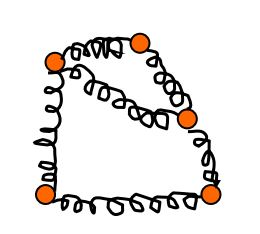
\includegraphics[scale=0.6]{bilder/graphfederfirst}\label{fig_graphfederfirst}
	}
	\hspace{1.0cm}%
	\subfigure[die Federn verschieben die Knoten]
	{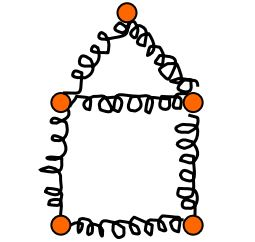
\includegraphics[scale=0.6]{bilder/graphfedersecond}\label{fig_graphfedersecond}
	}
	\hspace{1.0cm}%
	\subfigure[darstellung als Graph]
	{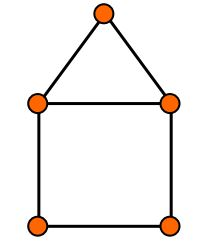
\includegraphics[scale=0.6]{bilder/graphfederthird}\label{fig_graphfederthird}
	}
	\\
	\caption[Darstellung als Stahlkugeln und Federn eines Graphen]{Darstellung als Stahlkugeln und Federn eines Graphen}
	\label{fig_testbild2}
\end{figure}
In diesem Kapitel werden die Grundlagen des Spring-Algorithmus erklärt, der im Kapitel 4 dazu verwendet wird um eine MetroMap ähnliche Darstellung des Höchstspannungsnetzes zu erhalten. Es geht um die Verwendung dieser Algorithmen und das grundsätzliche Vorgehen. Ebenso werden auf Unterschiede zwischen den meist verwendeten Spring-Embedder eingegangen.

\section{Spring-Embedder - allgemein}
\label{Kapitel_3_-_Unterkapitel_2}

Auf Kräfte basierte Algorithmen gehören zu den flexibelsten Methoden zur Berechnung eines simplen Layouts für ungerichtete Graphen. Diese Algorithmen, auch Spring-Embedder genannt, beruhen nur auf der zugrunde liegenden Struktur des Graphen. Zeichnungen des Graphen die aus diesen Algorithmen resultieren, neigen dazu sehr ästhetisch und symmetrisch zu sein. Zudem liefern sie meist einen überschneidungsfreie Darstellung des Graphen sofern dieser planar ist.[Spring Embedders and Force Directed GraphDrawing Algorithms] \\

Die folgenden Ausführungen stammen aus dem Buch \grqq Software-Practice and Experience, VOL. 21(1 1), 1129-1164"(November 1991).

 
Das Problem der Darstellung basiert auf der Platzierung der Kanten sowie
Knoten um eine möglichst ästhetische Zeichnung des
Graphen zu erhalten, die gut lesbar und verständlich ist. Die grundlegenden Kriterien für eine ästhetischen Zeichnung eines Graphen sind:
\begin{enumerate}
	\item die Knoten sollten gleichmäßig verteilt werden
	\item minimale Überschneidung der Kanten
	\item einheitliche Länge der Kanten
	\item möglichst symmetrisch
	\item alles soll sich innerhalb der Fläche befinden[Graph Drawing by Force-directed Placement].
\end{enumerate}   

Das heißt es ist leicht möglich die wichtigen Informationen des Graphen anhand einer visuellen Darstellung zu erhalten. Dazu gehören unter anderem die Erkennung von Verbindungen zwischen Knoten oder deren Lage. Dies ist vor allem wichtig bei einer MetroMap wo es darum geht schnell herauszufinden wie es möglich ist von einem Punkt zu einem anderen zu kommen. Um dies zu erreichen gibt es verschiedenste Ansätze. Diese müssen auf dem verwendeten Graphen anwendbar sein, sollten jedoch auch simpel und effizient sein.\\


Im Folgenden wird es um eine Erweiterung eines Verfahrens gehen, welches auf Grundlage des von Peter D. Eades entwickelten Algorithmus aus dem Jahre 1984 basiert. Er erklärt seine Metapher wie folgt:

\begin{quote}
	The basic idea is as follows. To embed [lay out] a graph we replace the
	vertices by steel rings and replace each edge with a spring to form a
	mechanical system . . . The vertices are placed in some initial layout and
	let go so that the spring forces on the rings move the system to a minimal
	energy state.
\end{quote}

Es geht demnach um ein Modell, indem die Knoten durch Stahlringe und die Kanten durch Federn repräsentiert werden. Durch die Federn wirken anschließend Kräfte auf die Kugeln ein, wodurch sich diese verschieben. Die Kugeln sollten jedoch vorher zufällig verteilt werden damit es mit diesem Vorgang zu einer besseren Lösung kommt. 
Das Verschieben der Kugeln durch die Federn passiert solange bis es zu einem sogenannten minimal-energy-state kommt. Das bedeutet, dass die Federn und Kugeln in einer Position befinden, indem die einwirkenden Kräfte der Federn keine Bewegung der Kugeln mehr zulassen. Dies ist meist erreicht sobald die Federn ihre optimale Länge erreicht haben, sie demnach keine weitere Kraft mehr auf die Kugeln wirken können. Es kommt jedoch nicht immer dazu. Es kann passieren, dass sich von zwei Federn, die noch nicht ihre optimale Länge haben, durch die Konstellation der Knoten ihre wirkende Kraft gegeneinander auflöst.\\

Die wirkenden Kräfte der Federn können nach belieben gewählt werden und müssen dabei nicht dem Hookeschem Gesetz entsprechen. Das hookesche Gesetz beschreibt die elastische Verformung von Festkörpern, wenn deren Verformung proportional zur einwirkenden Belastung ist[Wikipedia]. Es können demnach beliebige Definitionen, der wirkenden Kräfte der Federn, benutzt werden um ein gewünschtes Ergebnis zu erreichen. Ein weiterer Unterschied zur physikalischen Realität ist die Anwendung der Kraft auf die Knoten. Es können beliebige Knoten gewählt und auf diese, die gewünschte Kraft angewendet werden. Im Folgenden werden anziehende Kräfte zwischen jedem Knotenpaar, welches durch eine Kanten verbunden ist, angewendet. Abstoßende Kräfte wirken zwischen jedem Knoten, die nicht miteinander verbunden sind, demnach ebenso nicht durch eine Feder modelliert wurden. Das sind die Freiheiten des Verfahrens im Vergleich zur Realität. \\

Ein weiteres sehr ähnliches Verfahren, welches auf dem von Eades beruht ist der Algorithmus von Kamada und Kawai. Sie modellierten den Graphen ebenfalls als ein System von Federn, jedoch, im Vergleich zu Eades, hielten sich sie sich an das Hockesche Gesetz und versuchten dieses mit mehreren Differentialgleichungen zu lösen um ein verbessertes Layout zu erhalten. Eades hielt es für sehr wichtig, dass verbundene Knoten nah zueinander gezeichnet werden, demnach hat er ausschließlich anziehende Kräfte zwischen verbundenen Knoten berechnet. Kamada und Kawai haben hingegen ein weiteres Konzept eingefügt, welches auch anziehende Kräfte zwischen nicht verbundenen Knoten berechnet. Diese Kräfte sind proportional zur Länge des kürzesten Pfades der beiden Knoten. Das Problem der Zeichnung eines Graphen sahen Kamada und Kawai als das Vorgehen zur Reduzierung der noch zu wirkenden Kräfte der Federn in dem Graphen. Ist ein Zustand erreicht in dem die Summe der wirkenden Kräfte der Federn zum Tiefpunkt gekommen ist, so sind die Positionen und Abstände der Knoten nahe zu optimal gewählt. Sie definierten die komplette Energie des Graphen als: 

\begin{align}
	\sum_{\leq i < j\leq |V|}k_{p_{v_{i}}p_{v_{j}}}(|p_{v_{i}}-p_{v_{j}}|-l_{v_{i}v_{j}})^{2}
\end{align}

wobei $p_{v_{i}}$ die Position des Ringes oder Knotens $v_{i}$ ist, $k_{p_{v_{i}}p_{v_{j}}}$ ist die Feder-Konstante zwischen den Positionen $p_{v_{i}}$ und $p_{v_{j}}$ und $l_{v_{i}v_{j}}$ ist der optimale Abstand der beiden Knoten $v_{i}$ und $v_{j}$. Diese Energie wird reduziert durch das Lösen von Differentialgleichungen eines Knotens zur Findung einer besseren Position mit einer geringeren Menge an Energie im System.\\


 Die optimale Länge der Kanten $k$, die als Federn modelliert werden, wird durch die Anzahl der Knoten sowie der zur Verfügung stehender Fläche $A$ bestimmt:

\begin{align}
	k =
	C\sqrt{A / |V|}
\end{align}

\begin{align}
	A =
	W * L.
\end{align}

$W$ ist die Weite und $L$ die Länge der zugrunde liegenden Oberfläche, auf der, der Graph gezeichnet wird. Es ist
wichtig zu wissen wie diese Maße sind um eine bessere Verteilung der Knoten zu ermöglichen. Da die bessere Verteilung der Knoten zu einem ästhetischen Graphen führt möchte man die Oberfläche optimal nutzen. Wie weit Knoten voneinander entfernt sein sollten, wird demnach durch die Anzahl der Knoten und der Oberfläche bestimmt. Besonders wichtig ist es, dass die Knoten nicht zu nah aber auch nicht zu weit voneinander entfernt gezeichnet werden, denn beides führt zu einer Verschlechterung der Attraktivität des Graphen. $k = C\sqrt{A / |V|}$ führt dazu, dass sich die Knoten $|V|$ weit genug voneinander entfernt befinden um die Fläche gut zu nutzen und ebenso nah genug sind um die Ästhetik der Zeichnung zu bewahren. Die Konstante $C$ sollte experimentell gewählt werden, denn die Struktur eines Graphen kann stark variieren. Um dennoch in der Lage zu sein auf diese Schwankungen reagieren zu können kann man die Konstante $C > 1$ beliebig vergrößern um einen größeren optimalen Abstand zu erhalten oder bei $C < 1$ die Größe des Abstandes verringern. \\





Bildet die bisherige 
Platzierung der Kanten und Knoten einen planaren Graphen, so wird die neue die Platzierung in fast allen Fällen
auch planar sein. Ein Graph ist planar wenn sich keine Kanten überschneiden, diese Eigenschaft ist besonders gewollt um den resultierenden Graphen noch übersichtlicher zu gestalten.





\section{Spring-Embedder - Vorgehen}
\label{Kapitel_3_-_Unterkapitel_2}
%

\begin{algorithm}[t]
	\centering
	\caption[Spring-Algorithmus]{Spring-Algorithmus} \label{algo_1}
	\begin{algorithmic}[1]
		\REQUIRE \begin{math} G:= (V,E) \end{math}
		\ENSURE \begin{math} G:= (V,E) \end{math}
		\FOR{\begin{math}i:=1 \leq iterations \end{math}}
		\FOR{\begin{math}v_{i} \in V\end{math}}
		\STATE $d_{v_{i}} := 0;$
		\FOR{(\begin{math}v_{j} \in V\end{math})}
		\IF{$v_{i}\neq v_{j}$}
		\STATE $\Delta := p_{v_{i}} - p_{v_{j}};$
		\STATE $d_{v_{i}} := d_{v_{i}} + (\Delta / |\Delta|) \cdot f^{r}_{v_{i},v_{j}}(|\Delta|));$
		\ENDIF
		\ENDFOR
		\ENDFOR
		\newline
		\FOR{\begin{math}e_{v_{i},v_{j}} \in E\end{math}}
		\STATE $\Delta := p_{v_{i}} - p_{v_{j}};$
		\STATE $d_{v_{i}} := d_{v_{i}} - (\Delta / |\Delta|) \cdot f^{a}_{v_{i},v_{j}}(|\Delta|));$
		\STATE $d_{v_{j}} := d_{v_{j}} + (\Delta / |\Delta|) \cdot f^{a}_{v_{i},v_{j}}(|\Delta|));$
		\ENDFOR
		\newline
		\FOR{\begin{math}v_{i} \in V\end{math}}
		\STATE $p_{v_{i}} := p_{v_{i}} + ( d_{v_{i}}/ |d_{v_{i}}|) \cdot min ( d_{v_{i}}, t );$
		\STATE $p_{v_{i}}^{x} := min(W/2, max(-W/2, p_{v_{i}}^{x}));$
		\STATE $p_{v_{i}}^{y} := min(L/2, max(-L/2, p_{v_{i}}^{y}))$
		\ENDFOR
		\STATE $t:= cool(t)$
		\ENDFOR
	\end{algorithmic}
\end{algorithm}

Zwischen jedem Knotenpaar $v_{i},v_{j} \in V$ wird eine abstoßende Kraft \begin{math} f^{r}_{v_{i},v_{j}}  \end{math} berechnet.   Alle
benachbarten Knoten erhalten eine anziehende Kraft \begin{math} f^{a}_{v_{i},v_{j}} \end{math}. Zwei Knoten \begin{math} v_{i},v_{j} \in V \end{math}sind benachbart wenn \begin{math} e_{v_{i},v_{j}} \in E \end{math} ist. Das führt dazu, dass verbundene Knoten näher zusammen
gezeichnet werden, während sie noch immer einen gewissen Abstand zueinander
haben. Der Algorithmus geht dabei in drei Schritten vor:

\begin{enumerate}
	\item zwischen jedem Knotenpaar die abstoßende Kraft berechnen
	\item benachbarten Knoten eine anziehende Kraft zuweisen
	\item jeden Knoten seiner neuen Kraft nach bewegen.
\end{enumerate} 
Diese drei Schritte werden werden so oft wiederholt bis keine weitere Bewegung mehr stattfindet.
Die Funktionen \begin{math} f^{a}_{v_{i},v_{j}} \end{math} und \begin{math} f^{r}_{v_{i},v_{j}} \end{math} sind wie folgt definiert:


\begin{align}
	f^{a}_{v_{i},v_{j}} (x) =
	x^{2}/k
\end{align}

\begin{align}
	f^{r}_{v_{i},v_{j}} (x) =
	-k^{2}/x.
\end{align}


\begin{figure}[t]
	\centering
	\subfigure[anziehende Kraft $f^{a}$ zwischen dem dritten und vierten Knoten]
	{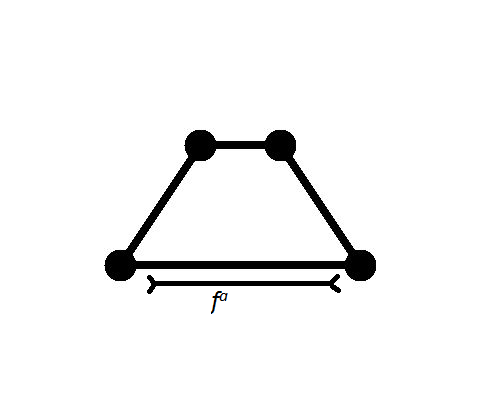
\includegraphics[scale=0.3]{bilder/kraftfa}\label{fig_kraftfa}
	}
	\hspace{1.0cm}%
	\subfigure[abstoßende Kraft $f^{r}$ zwischen dem ersten und vierten Knoten]
	{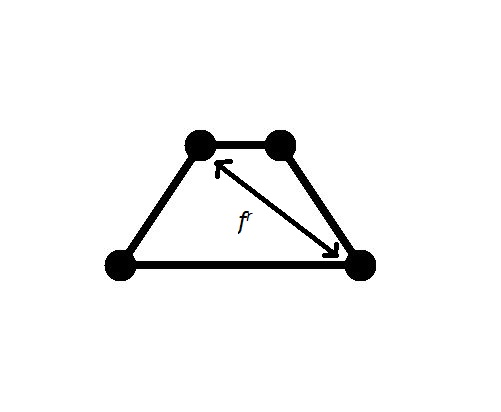
\includegraphics[scale=0.3]{bilder/kraftfr}\label{fig_kraftfr}
	}
	\hspace{1.0cm}%
	\subfigure[die wirkenden Kräfte lösen sich auf]
	{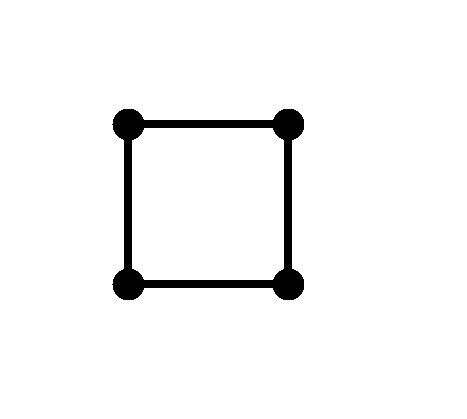
\includegraphics[scale=0.3]{bilder/standardgraph}\label{fig_standardgraph}
	}
	\\
	\caption[Wirkende Kräfte im Graphen]{Wirkende Kräfte im Graphen}
	\label{fig_testbild2}
\end{figure} 


Der Vektor $d_{v_{i}}$ gibt an in welcher Richtung der Knoten $v_{i}$ bewegt wird. Während der Vektor $p_{v_{i}}$ auf die momentane Position des Knoten $v_{i}$ zeigt. Der Vektor $\Delta$ ist die Differenz zwischen $p_{v_{i}}$ und $p_{v_{j}}$, der Richtungsvektor von $v_{i}$ nach $v_{j}$. Die Variable $iterations$ gibt die Anzahl der Durchläufe an. Bei jedem neuen Durchlauf wird der Vektor  $d_{v}$  eines jeden Knotens $v$ auf 0 gesetzt. Mit zwei For-Schleifen geht man jede Knotenkombination durch und berechnet die abstoßende Kraft $f^{r}_{v_{i},v_{j}}$ mithilfe der Länge des $\Delta$ Vektors. Anschließend wird der Bewegungsvektor auf den Einheitsvektor von $\Delta$ multipliziert mit der berechneten Kraft gesetzt. Dadurch drücken sich die Knoten direkt voneinander weg. \\

Der zweite Schritt besteht darin die anziehenden Kräfte zwischen den benachbarten Knoten zu berechnen. Dazu wird jede Kante einmal durchgegangen und der Bewegungsvektor von jedem betroffenen Knoten wird wie bei der abstoßenden Kraft aufaddiert. \\

Im letzten Schritt des Algorithmus werden die Knoten nun in Richtung ihres Bewegungsvektors bewegt. Es wird darauf geachtet, dass die Knoten dabei nicht das Bild verlassen. Die Variable $t$ ermöglicht es, am Anfang viel Bewegung der Knoten zuzulassen und dies immer weiter einzuschränken, damit mit der Graph mit jeder Iteration feiner wird. Die Funktion $cool(t)$ regelt dabei wie weit sich jeder Knoten in der nächsten Iteration maximal bewegen darf. $t$ könnte zum Beispiel bei der Länge des Bildes starten und sich nach jeder Iteration um ein Zehntel mit $cool(t)$ kürzen. Nach 10 Iterationen wären dadurch keine weiteren Bewegungen der Knoten mehr möglich.


\section{Spring-Algorithmus - Erweiterbarkeit}
\label{Kapitel_3_-_Unterkapitel_3}   
%